\documentclass[conference]{IEEEtran}
\usepackage{cite}
\usepackage{amsmath,amssymb,amsfonts}
\usepackage{graphicx}
\usepackage{booktabs}
\usepackage{pgfplots}
\usepgfplotslibrary{groupplots}
\pgfplotsset{compat=1.17}
\usepackage{xcolor}
\usepackage{flafter}
\usepackage{placeins}

\begin{document}

\title{Particle Swarm Optimization for Continuous Benchmark Functions:\\
Parameter Influence, Tuning and Hybridization with Local Search}

\author{\IEEEauthorblockN{Martinas Ioana Maria and Zaborila Eduard Andrei}
\IEEEauthorblockA{\textit{Master Program, Nature-Inspired Methods (NIM)}\\
\textit{Faculty of Computer Science, ``Alexandru Ioan Cuza'' University, Ia\c{s}i}}}

\maketitle

\begin{abstract}
This report presents a real-valued Particle Swarm Optimization (PSO)
algorithm applied to the Rastrigin, Griewangk, Rosenbrock and Michalewicz
benchmark functions in 2, 30 and 100 dimensions. A one-factor-at-a-time
study on 30-dimensional instances quantifies the influence of swarm size,
inertia weight, inertia schedule, acceleration coefficients, velocity limit
and topology on convergence. The results agree with the theoretical
stability region of PSO: settings outside it ($w\geq0.9$, $c_1=c_2=2$)
consistently fail, and removing the social term is catastrophic. Based on
the study, a tuned configuration ($v_{\max}=0.05(b-a)$, $c_1=2$, $c_2=1$),
a hybrid PSO with coordinate-wise local search applied to the global
best, and an enhanced hybrid that adds stagnation-triggered partial
restarts, an arithmetic crossover between personal bests and a periodic
local search were designed. With 30 independent runs per instance and a
budget that grows with dimension, the enhanced hybrid solves Rastrigin
exactly in 30 and 100 dimensions (mean $0.0$), lowers the 30-dimensional
Rosenbrock error from 15.6 to 0.53, the 100-dimensional Rosenbrock error
from 95.5 to 58.9, the 100-dimensional Griewangk error from 0.366 to
0.0028, and reaches 93\% of the best-known optimum on 100-dimensional
Michalewicz. Almost all improvements are statistically significant
(Mann--Whitney U test, $p<0.05$; $p<10^{-5}$ in most cases). Compared with
the Hill Climbing and hybrid GA of a previous study, the enhanced hybrid
PSO matches or beats GA+HC on the multimodal functions, while GA+HC keeps
an edge on the non-separable Rosenbrock.
\end{abstract}

\begin{IEEEkeywords}
particle swarm optimization, numerical optimization, parameter tuning,
hybrid metaheuristics, local search, benchmark functions
\end{IEEEkeywords}

%=====================================================================
\section{Introduction}
%=====================================================================
Particle Swarm Optimization (PSO), introduced by Kennedy and Eberhart in
1995~\cite{kennedy1995,eberhart1995}, is a population-based stochastic
optimizer inspired by the collective motion of bird flocks. Each candidate
solution, called a \emph{particle}, moves through the search space with a
velocity that is attracted towards its own best position (cognitive
component) and towards the best position found by its neighbors (social
component). Unlike Genetic Algorithms (GA)~\cite{holland1975,goldberg1989},
PSO has no selection, crossover or mutation; information is shared only
through attraction. PSO is therefore simple, naturally suited to
continuous domains and inexpensive per iteration. Comprehensive overviews
of PSO, its theory and its many variants can be found
in~\cite{kennedy2001,poli2007,engelbrecht2007,bonyadi2017}, and an early
comparison between PSO and evolutionary algorithms is given
in~\cite{angeline1998}.

This work continues a previous assignment (H1), in which Hill Climbing (HC)
and a binary Genetic Algorithm~\cite{michalewicz1996} hybridized with
HC~\cite{talbi2002} were applied to the same benchmarks. The goals of this
report are:
\begin{itemize}
\item to implement PSO with real-valued representation for four benchmark
functions in 2, 30 and 100 dimensions, with at least five-decimal
precision;
\item to analyze, experimentally and in light of known theory, how each
PSO parameter influences convergence;
\item to use the findings to build an improved configuration and a hybrid
PSO with local search, mirroring the GA+HC hybridization of H1;
\item to compare PSO with the HC and GA results of H1.
\end{itemize}

Section~\ref{sec:problem} describes the benchmarks, Section~\ref{sec:pso}
the algorithm and its variants, Section~\ref{sec:setup} the protocol,
Section~\ref{sec:study} the parameter study, Section~\ref{sec:main} the
main results and the comparison with H1, Section~\ref{sec:discussion} the
discussion and Section~\ref{sec:conclusion} the conclusions.

%=====================================================================
\section{Benchmark Problems}\label{sec:problem}
%=====================================================================
All problems are minimized over $[a,b]^n$.

\textbf{Rastrigin}~\cite{rastrigin1974,muhlenbein1991} is separable and
highly multimodal, with a regular grid of local minima spaced about one
unit apart:
\begin{equation}
\begin{split}
f_1(\mathbf{x}) = 10n + \sum_{i=1}^{n}\Big[&x_i^2 - 10\cos(2\pi x_i)\Big],\\
&x_i\in[-5.12,5.12].
\end{split}
\end{equation}

\textbf{Griewangk}~\cite{griewank1981} has many local minima whose number
grows exponentially with $n$, but whose relative depth decreases with
dimension; its domain is very wide compared with the region of interest:
\begin{equation}
f_2(\mathbf{x}) = \sum_{i=1}^{n}\frac{x_i^2}{4000}
-\prod_{i=1}^{n}\cos\!\left(\frac{x_i}{\sqrt{i}}\right)+1,
\quad x_i\in[-600,600].
\end{equation}

\textbf{Rosenbrock}~\cite{rosenbrock1960} is non-separable, with a narrow
curved valley that is easy to find and hard to follow:
\begin{equation}
\begin{split}
f_3(\mathbf{x}) = \sum_{i=1}^{n-1}\Big[&100(x_{i+1}-x_i^2)^2+(1-x_i)^2\Big],\\
&x_i\in[-2.048,2.048].
\end{split}
\end{equation}

\textbf{Michalewicz}~\cite{michalewicz1996} ($m=10$) is separable, but has
$n!$ local optima, large flat plateaus and very narrow, steep valleys,
which make it deceptive for population methods:
\begin{equation}
f_4(\mathbf{x}) = -\sum_{i=1}^{n}\sin(x_i)\,
\sin^{2m}\!\left(\frac{i\,x_i^2}{\pi}\right),
\quad x_i\in[0,\pi].
\end{equation}

The global minima are listed in Table~\ref{tab:optima}; for Michalewicz in
30 and 100 dimensions, the values are approximate best-known values.

\begin{table}[t]
\centering
\caption{Global minima of the benchmark functions}
\label{tab:optima}
\begin{tabular}{lccc}
\toprule
Function & $n=2$ & $n=30$ & $n=100$\\
\midrule
Rastrigin, Griewangk, Rosenbrock & 0 & 0 & 0\\
Michalewicz & $-1.8013$ & $\approx-29.63$ & $\approx-99.28$\\
\bottomrule
\end{tabular}
\end{table}

%=====================================================================
\section{Particle Swarm Optimization}\label{sec:pso}
%=====================================================================
\subsection{Update equations}
A swarm of $S$ particles is maintained. Particle $i$ has position
$\mathbf{x}_i$, velocity $\mathbf{v}_i$, personal best $\mathbf{p}_i$ and
neighborhood leader $\mathbf{l}_i$. At each iteration:
\begin{align}
\mathbf{v}_i &\leftarrow w\,\mathbf{v}_i
 + c_1\,\mathbf{r}_1\odot(\mathbf{p}_i-\mathbf{x}_i)
 + c_2\,\mathbf{r}_2\odot(\mathbf{l}_i-\mathbf{x}_i),\label{eq:v}\\
\mathbf{x}_i &\leftarrow \mathbf{x}_i+\mathbf{v}_i,\label{eq:x}
\end{align}
where $\mathbf{r}_1,\mathbf{r}_2\sim U(0,1)^n$, $\odot$ is the
element-wise product, $w$ is the inertia weight, and $c_1$, $c_2$ are the
cognitive and social coefficients.

\subsection{Velocity clamping and boundaries}
Velocities are clamped to $[-v_{\max},v_{\max}]$ with
$v_{\max}=\alpha(b-a)$. A particle that leaves the domain is clipped to the
boundary, and its velocity on that dimension is set to zero (``absorbing
wall'').

\subsection{Inertia, topology and stability}
Two inertia schedules are supported: constant $w=0.7298$, and linear decay
$w(t)=w_{\max}-(w_{\max}-w_{\min})\,t/(T-1)$ with
$0.9\to0.4$~\cite{shi1998,shi1999}. In the \emph{global} topology,
$\mathbf{l}_i$ is the swarm's best position; in the \emph{ring} topology,
$\mathbf{l}_i$ is the best of
$\{\mathbf{p}_{i-1},\mathbf{p}_i,\mathbf{p}_{i+1}\}$~\cite{kennedy2002,mendes2004}.

The baseline $w=0.7298$, $c_1=c_2=1.49618$ is equivalent to Clerc and
Kennedy's constriction~\cite{clerc2002,eberhart2000,shi1998param}. A
standard sufficient condition for order-1 and order-2 stability of the
particle dynamics is~\cite{poli2009}
\begin{equation}
c_1+c_2 < \frac{24(1-w^2)}{7-5w},\qquad |w|<1.\label{eq:stab}
\end{equation}
For $c_1+c_2=2.992$, (\ref{eq:stab}) holds only for $w\lesssim0.786$, and
for $w=0.7298$ the bound is $3.35$: the baseline lies just inside the
stable region. Other convergence analyses of the particle
dynamics~\cite{trelea2003,vandenbergh2006} lead to similar parameter
recommendations.

\subsection{Tuned and hybrid variants}
Based on the parameter study (Section~\ref{sec:study}), three additional
variants were defined:
\begin{itemize}
\item \textbf{tuned}: baseline with $\alpha=0.05$, $c_1=2.0$, $c_2=1.0$.
Since $c_1+c_2=3<3.35$, it remains stable.
\item \textbf{tuned\_hybrid}: the tuned PSO followed by a local search that
adjusts one variable at a time, applied to the final global best. This
search works the same way as the HC used in the GA+HC hybrid of H1, but on
real numbers instead of bits. It belongs to the family of coordinate-wise
direct search methods~\cite{hooke1961}, and combining it with PSO follows
the usual idea of mixing a global search with a local one~\cite{talbi2002}.
It uses an initial step of $0.01(b-a)$ that is reduced by half when no
coordinate move improves, down to $10^{-7}$, with a cap of 20\,000
evaluations.
\item \textbf{tuned\_hybrid2} (enhanced hybrid): the tuned PSO with three
extra parts that work together, plus the same final local search. It uses a
larger swarm ($S=80$) and $v_{\max}=0.07(b-a)$. (i) A \emph{stagnation
restart}: when the global best does not improve for 120 iterations, the
worst 20\% of the particles are reinitialized, half uniformly in the domain
and half in a neighborhood of the global best; the global best itself is
never lost. This restores diversity and lets the swarm escape the basins
where Rastrigin stagnates. (ii) An \emph{arithmetic crossover} between
personal bests, inspired by the GA of H1: with probability $0.3$ per
iteration, two good personal bests are blended and the child replaces the
worst particle if it is better. This recombination is particularly useful
on the non-separable Rosenbrock. (iii) A \emph{periodic local search} on the
global best every 500 iterations, and a longer final local search (up to
100\,000 evaluations). These extra searches make this variant more accurate
but also more expensive (see the cost discussion in
Section~\ref{sec:main}).
\end{itemize}

%=====================================================================
\section{Experimental Setup}\label{sec:setup}
%=====================================================================
\textbf{Main experiment.} Every function was run in $n\in\{2,30,100\}$
with 30 independent runs per instance and $S=50$ (baseline, tuned and
tuned\_hybrid). The number of iterations grows with dimension,
$T\in\{1000,3000,6000\}$, giving $50\,050$, $150\,050$ and $300\,050$
evaluations per run for those variants; the local search of tuned\_hybrid
adds at most 20\,000 evaluations. The enhanced hybrid (tuned\_hybrid2) uses
$S=80$ and stronger local search, so it uses more evaluations (see
Section~\ref{sec:main}). Run $r$ of every variant uses the same random seed
($1000+r$), so all variants are compared on common random numbers.

\textbf{Parameter study.} On all four functions with $n=30$, one parameter
was varied at a time while the others kept their baseline values
(Table~\ref{tab:params}), with 10 runs of $T=500$ iterations each. The
values studied were $S\in\{10,30,50,100\}$; $w\in\{0.2,0.5,0.7298,0.9,
1.1\}$; constant versus decreasing inertia;
$(c_1,c_2)\in\{(0.5,2.5),(1.5,1.5),(2,2),(2.5,0.5),(0,2),(2,0)\}$;
$\alpha\in\{0.05,0.1,0.2,0.5,1\}$; and global versus ring topology.

\textbf{Statistics and environment.} The minimum, mean, maximum and
standard deviation of the final values are reported. Variants are
compared with the two-sided Mann--Whitney U test~\cite{mann1947} at the
0.05 level.

\begin{table}[t]
\centering
\caption{Baseline PSO configuration}
\label{tab:params}
\begin{tabular}{ll}
\toprule
Parameter & Value\\
\midrule
Swarm size $S$ & 50\\
Iterations $T$ & 1000 / 3000 / 6000 for $n=2/30/100$\\
Inertia $w$ & 0.7298 (constant)\\
$c_1$, $c_2$ & 1.49618, 1.49618\\
$v_{\max}$ & $0.2\,(b-a)$\\
Topology & global\\
\bottomrule
\end{tabular}
\end{table}

%=====================================================================
\section{Parameter Study}\label{sec:study}
%=====================================================================
\subsection{Swarm size}
A very small swarm ($S=10$) is clearly insufficient
(Fig.~\ref{fig:swarm}): Griewangk degrades to $0.90$ compared with $0.016$
at $S=50$. The largest swarm, $S=100$, gives the best mean on all four
functions (Rastrigin 46.27, Griewangk 0.0103, Rosenbrock 23.46, Michalewicz
$-25.36$), but it also uses twice as many evaluations. Between $S=30$ and
$S=50$ the differences are within one standard deviation; for Rastrigin,
for example, 60.69 and 63.38 with std of about 13--17.

\begin{figure*}[t]
\centering
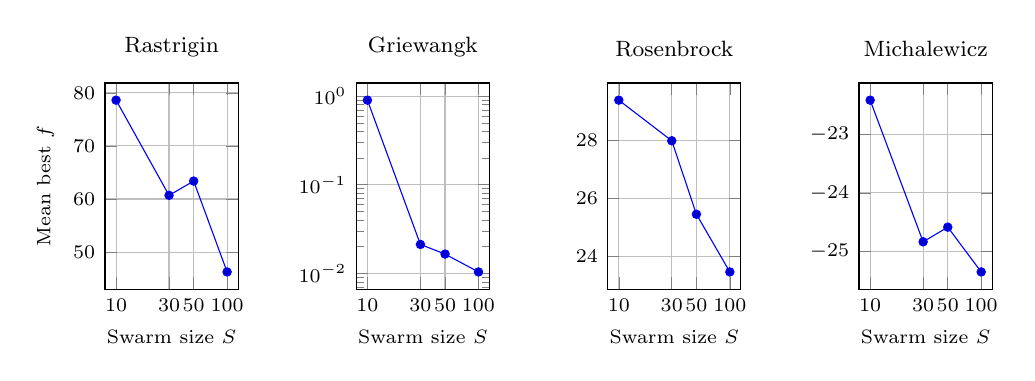
\begin{tikzpicture}
\begin{groupplot}[
  group style={group size=4 by 1, horizontal sep=1.5cm},
  width=0.27\textwidth, height=4.2cm,
  xmode=log, xtick={10,30,50,100}, xticklabels={10,30,50,100},
  xlabel={Swarm size $S$}, grid=major,
  every axis plot/.append style={mark=*, mark size=1.5pt},
  title style={font=\footnotesize}, tick label style={font=\scriptsize},
  label style={font=\scriptsize}]
\nextgroupplot[title=Rastrigin, ylabel={Mean best $f$}]
\addplot coordinates {(10,78.615) (30,60.692) (50,63.379) (100,46.265)};
\nextgroupplot[title=Griewangk, ymode=log]
\addplot coordinates {(10,0.90158) (30,0.02115) (50,0.01646) (100,0.01034)};
\nextgroupplot[title=Rosenbrock]
\addplot coordinates {(10,29.395) (30,27.992) (50,25.455) (100,23.463)};
\nextgroupplot[title=Michalewicz]
\addplot coordinates {(10,-22.408) (30,-24.839) (50,-24.587) (100,-25.356)};
\end{groupplot}
\end{tikzpicture}
\caption{Influence of swarm size ($n=30$, 500 iterations, 10 runs).}
\label{fig:swarm}
\end{figure*}

\subsection{Inertia weight}
The inertia weight is the most influential parameter (Fig.~\ref{fig:w});
$w=0.7298$ is the best value on all four functions. Small values make the
swarm lose momentum too early, so it collapses onto the first good region:
on Griewangk the mean is $0.0165$ at $w=0.7298$, but $2.79$ at $w=0.5$ and
$38.7$ at $w=0.2$. Values beyond the stability limit $w\approx0.786$ of
(\ref{eq:stab}) are even worse. At $w=0.9$ the trajectories have unbounded
variance, and at $w=1.1$ velocities grow geometrically; only velocity
clamping keeps the particles inside the domain. The result is a bounded
random walk: Rastrigin 180.8 and 241.7, Rosenbrock 121.2 and 450.5,
Michalewicz $-12.3$ and $-10.7$.

\begin{figure*}[t]
\centering
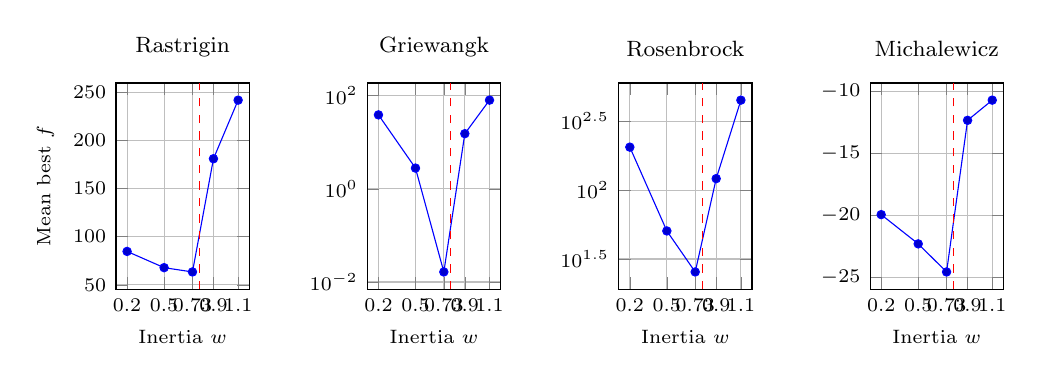
\begin{tikzpicture}
\begin{groupplot}[
  group style={group size=4 by 1, horizontal sep=1.5cm},
  width=0.27\textwidth, height=4.2cm,
  xlabel={Inertia $w$}, xtick={0.2,0.5,0.73,0.9,1.1},
  xticklabels={0.2,0.5,0.73,0.9,1.1},
  grid=major,
  every axis plot/.append style={mark=square*, mark size=1.5pt},
  title style={font=\footnotesize}, tick label style={font=\scriptsize},
  label style={font=\scriptsize}]
\nextgroupplot[title=Rastrigin, ylabel={Mean best $f$}]
\addplot coordinates {(0.2,84.681) (0.5,67.829) (0.7298,63.379) (0.9,180.848) (1.1,241.662)};
\draw[dashed,red] ({axis cs:0.786,1}|-{rel axis cs:0,0}) -- ({axis cs:0.786,1}|-{rel axis cs:0,1});
\nextgroupplot[title=Griewangk, ymode=log]
\addplot coordinates {(0.2,38.69342) (0.5,2.79001) (0.7298,0.01646) (0.9,15.27777) (1.1,80.17860)};
\draw[dashed,red] ({axis cs:0.786,1}|-{rel axis cs:0,0}) -- ({axis cs:0.786,1}|-{rel axis cs:0,1});
\nextgroupplot[title=Rosenbrock, ymode=log]
\addplot coordinates {(0.2,205.227) (0.5,50.525) (0.7298,25.455) (0.9,121.207) (1.1,450.472)};
\draw[dashed,red] ({axis cs:0.786,1}|-{rel axis cs:0,0}) -- ({axis cs:0.786,1}|-{rel axis cs:0,1});
\nextgroupplot[title=Michalewicz]
\addplot coordinates {(0.2,-19.950) (0.5,-22.316) (0.7298,-24.587) (0.9,-12.323) (1.1,-10.691)};
\draw[dashed,red] ({axis cs:0.786,1}|-{rel axis cs:0,0}) -- ({axis cs:0.786,1}|-{rel axis cs:0,1});
\end{groupplot}
\end{tikzpicture}
\caption{Influence of the inertia weight ($n=30$). The dashed line marks the
theoretical stability limit $w\approx0.786$ for $c_1+c_2=2.992$.}
\label{fig:w}
\end{figure*}

\subsection{Constant versus decreasing inertia}
With the schedule $0.9\to0.4$, $w$ exceeds the stability limit during the
first $\approx23\%$ of the iterations. This extra early exploration helps on
Rastrigin, where the mean falls from 63.38 to 51.77, but it wastes budget on
the other three functions (Table~\ref{tab:decay}).

\begin{table}[t]
\centering
\caption{Inertia schedule (mean $\pm$ std, $n=30$, 10 runs)}
\label{tab:decay}
\begin{tabular}{lcc}
\toprule
Function & $w=0.7298$ (fixed) & $w:0.9\to0.4$\\
\midrule
Rastrigin   & $63.379\pm16.554$ & $\mathbf{51.771}\pm16.356$\\
Griewangk   & $\mathbf{0.0165}\pm0.0186$ & $0.0340\pm0.0407$\\
Rosenbrock  & $\mathbf{25.455}\pm1.375$ & $26.737\pm1.700$\\
Michalewicz & $\mathbf{-24.587}\pm1.464$ & $-22.441\pm1.741$\\
\bottomrule
\end{tabular}
\end{table}

\subsection{Acceleration coefficients}
Table~\ref{tab:c} shows three regimes. A \emph{purely cognitive} swarm
($c_2=0$) is by far the worst on every function (Rosenbrock 5019.5,
Griewangk 506.1): without social information each particle performs an
isolated search, which shows that cooperation is the core mechanism of
PSO. A \emph{purely social} swarm ($c_1=0$) converges prematurely, for
example to 88.6 on Rastrigin. The pair $(2,2)$ doesn't respect (\ref{eq:stab}),
since $4>3.35$, and degrades all functions. Among stable settings, the
balanced pair $(1.5,1.5)$ is best on Griewangk, Rosenbrock and Michalewicz.
On Rastrigin, however, the cognitively biased pair $(2.5,0.5)$ halves the
error (29.79, std 5.43): a weak social pull keeps particles exploring their
own basins for longer. This is consistent with time-varying acceleration
schemes~\cite{ratnaweera2004}, which use a large cognitive and a small
social coefficient early in the run to enhance exploration.

\begin{table}[t]
\centering
\caption{Acceleration coefficients (mean, $n=30$, 10 runs). Best per
column in bold.}
\label{tab:c}
\setlength{\tabcolsep}{4pt}
\begin{tabular}{lrrrr}
\toprule
$(c_1,c_2)$ & Rastrigin & Griewangk & Rosenbrock & Michalewicz\\
\midrule
$(0.5,2.5)$ & 73.24 & 0.909 & 31.65 & $-23.62$\\
$(1.5,1.5)$ & 61.49 & \textbf{0.020} & \textbf{25.59} & $\mathbf{-25.69}$\\
$(2.0,2.0)$ & 108.49 & 2.333 & 41.19 & $-17.80$\\
$(2.5,0.5)$ & \textbf{29.79} & 1.028 & 41.31 & $-23.18$\\
$(0.0,2.0)$ & 88.59 & 0.250 & 26.96 & $-22.93$\\
$(2.0,0.0)$ & 355.71 & 506.069 & 5019.47 & $-9.44$\\
\bottomrule
\end{tabular}
\end{table}

\subsection{Velocity limit}
The value $\alpha=1$ is the worst setting on all four functions
(Fig.~\ref{fig:vmax}). On Rastrigin and Michalewicz the effect is
monotonic: $\alpha=0.05$ reduces by half the Rastrigin error (31.34 versus 63.38) and
gives the best Michalewicz value of the study ($-26.77$). Short steps force
a fine search around promising regions and prevent particles from being
thrown into distant basins. Rosenbrock is best at $\alpha=0.1$ (24.47),
while Griewangk is almost insensitive in the range $0.05$--$0.5$, where the
differences are smaller than the standard deviation.

\begin{figure*}[t]
\centering
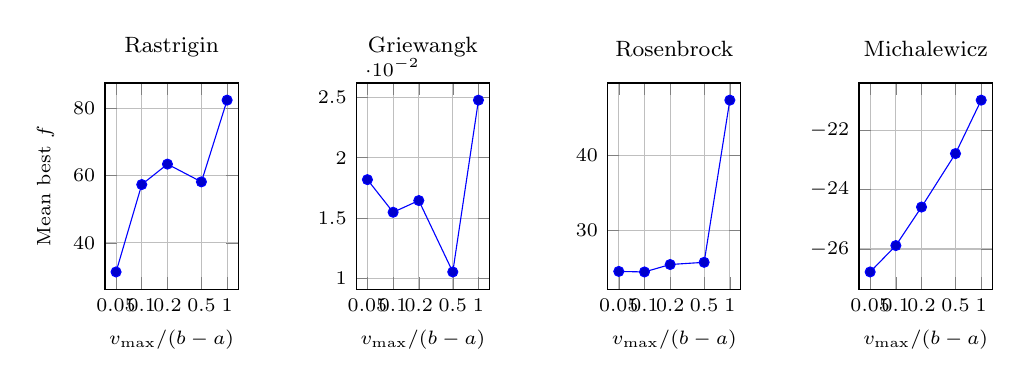
\begin{tikzpicture}
\begin{groupplot}[
  group style={group size=4 by 1, horizontal sep=1.5cm},
  width=0.27\textwidth, height=4.2cm,
  xmode=log, xtick={0.05,0.1,0.2,0.5,1}, xticklabels={0.05,0.1,0.2,0.5,1},
  xlabel={$v_{\max}/(b-a)$}, grid=major,
  every axis plot/.append style={mark=triangle*, mark size=1.8pt},
  title style={font=\footnotesize}, tick label style={font=\scriptsize},
  label style={font=\scriptsize}]
\nextgroupplot[title=Rastrigin, ylabel={Mean best $f$}]
\addplot coordinates {(0.05,31.341) (0.1,57.310) (0.2,63.379) (0.5,58.106) (1,82.389)};
\nextgroupplot[title=Griewangk]
\addplot coordinates {(0.05,0.01819) (0.1,0.01549) (0.2,0.01646) (0.5,0.01055) (1,0.02477)};
\nextgroupplot[title=Rosenbrock]
\addplot coordinates {(0.05,24.537) (0.1,24.467) (0.2,25.455) (0.5,25.748) (1,47.308)};
\nextgroupplot[title=Michalewicz]
\addplot coordinates {(0.05,-26.775) (0.1,-25.886) (0.2,-24.587) (0.5,-22.784) (1,-20.982)};
\end{groupplot}
\end{tikzpicture}
\caption{Influence of the velocity limit ($n=30$, 500 iterations, 10 runs).}
\label{fig:vmax}
\end{figure*}

\subsection{Topology}
The ring topology is clearly better on Rastrigin (47.90 versus 63.38, with
half the standard deviation), where slower information diffusion preserves
diversity. It is worse on the other three functions, most visibly on
Griewangk (0.196 versus 0.0165), because within 500 iterations good
information has not yet reached the whole swarm~\cite{kennedy2002,bratton2007}
(Table~\ref{tab:topo}).

\begin{table}[t]
\centering
\caption{Topology (mean $\pm$ std, $n=30$, 10 runs)}
\label{tab:topo}
\begin{tabular}{lcc}
\toprule
Function & Global & Ring\\
\midrule
Rastrigin   & $63.379\pm16.554$ & $\mathbf{47.902}\pm8.444$\\
Griewangk   & $\mathbf{0.0165}\pm0.0186$ & $0.1958\pm0.0751$\\
Rosenbrock  & $\mathbf{25.455}\pm1.375$ & $26.695\pm0.419$\\
Michalewicz & $\mathbf{-24.587}\pm1.464$ & $-22.777\pm1.040$\\
\bottomrule
\end{tabular}
\end{table}

%=====================================================================
\section{Main Results}\label{sec:main}
%=====================================================================
\subsection{Baseline PSO}
Table~\ref{tab:main} reports the baseline results. In two dimensions PSO is
essentially exact: Rastrigin, Rosenbrock and Michalewicz reach the optimum
in all 30 runs with zero variance, and on Griewangk only a few runs stop in
a neighboring local minimum (maximum 0.0074).

In 30 dimensions, Griewangk is solved well (mean 0.0204) and Rosenbrock
reaches 15.62. Rastrigin stays high (about 59), because there the swarm
stagnates in a local basin, and more iterations alone cannot escape it.
Michalewicz reaches 85\% of the best-known value. In 100 dimensions all
errors grow, and the running time increases to about 4\,s per run.

\begin{table*}[t]
\centering
\caption{Baseline PSO (30 runs, $S=50$)}
\label{tab:main}
\begin{tabular}{llrrrrrr}
\toprule
Function & $n$ & Min & Mean & Max & Std & Evaluations & Time/run (s)\\
\midrule
Rastrigin   & 2   & 0.00000 & 0.00000 & 0.00000 & 0.00000 & 50\,050 & 0.03\\
Griewangk   & 2   & 0.00000 & 0.00125 & 0.00740 & 0.00275 & 50\,050 & 0.04\\
Rosenbrock  & 2   & 0.00000 & 0.00000 & 0.00000 & 0.00000 & 50\,050 & 0.03\\
Michalewicz & 2   & $-1.80130$ & $-1.80130$ & $-1.80130$ & 0.00000 & 50\,050 & 0.03\\
\midrule
Rastrigin   & 30  & 28.85380 & 59.10041 & 87.55603 & 13.39213 & 150\,050 & 0.43\\
Griewangk   & 30  & 0.00000 & 0.02040 & 0.07635 & 0.02142 & 150\,050 & 0.56\\
Rosenbrock  & 30  & 12.54489 & 15.61683 & 20.52056 & 2.04120 & 150\,050 & 0.62\\
Michalewicz & 30  & $-27.80665$ & $-25.21621$ & $-21.89808$ & 1.60151 & 150\,050 & 0.64\\
\midrule
Rastrigin   & 100 & 197.00151 & 281.64353 & 376.09287 & 42.76870 & 300\,050 & 2.43\\
Griewangk   & 100 & 0.00000 & 0.36574 & 1.94079 & 0.46674 & 300\,050 & 3.31\\
Rosenbrock  & 100 & 77.71005 & 95.47126 & 193.61131 & 24.43257 & 300\,050 & 3.87\\
Michalewicz & 100 & $-87.22997$ & $-83.80107$ & $-77.86669$ & 2.11889 & 300\,050 & 3.97\\
\bottomrule
\end{tabular}
\end{table*}

\subsection{Tuned and hybrid variants}
Table~\ref{tab:var} and Fig.~\ref{fig:var} compare the four variants. In
2 dimensions all variants are exact; on Griewangk, the tuned variants
remove the few failed baseline runs (mean 0.00000 versus 0.00125,
$p=0.011$).

\begin{table*}[t]
\centering
\caption{Comparison of PSO variants (mean $\pm$ std, 30 runs). $^{+}$ / $^{-}$:
significantly better / worse than baseline (Mann--Whitney, $p<0.05$).
Best mean in bold.}
\label{tab:var}
\begin{tabular}{llcccc}
\toprule
Function & $n$ & baseline & tuned & tuned\_hybrid & tuned\_hybrid2\\
\midrule
Rastrigin   & 30  & $59.100\pm13.392$ & $30.877\pm7.562^{+}$ & $30.877\pm7.562^{+}$ & $\mathbf{0.000}\pm0.000^{+}$\\
Griewangk   & 30  & $0.0204\pm0.0214$ & $0.0155\pm0.0196$ & $0.0155\pm0.0196$ & $\mathbf{0.0091}\pm0.0113^{+}$\\
Rosenbrock  & 30  & $15.617\pm2.041$ & $20.548\pm1.548^{-}$ & $12.910\pm1.534^{+}$ & $\mathbf{0.535}\pm1.355^{+}$\\
Michalewicz & 30  & $-25.216\pm1.602$ & $-26.895\pm1.029^{+}$ & $-27.311\pm0.764^{+}$ & $\mathbf{-27.774}\pm0.597^{+}$\\
\midrule
Rastrigin   & 100 & $281.644\pm42.769$ & $106.767\pm22.229^{+}$ & $93.924\pm21.534^{+}$ & $\mathbf{0.000}\pm0.000^{+}$\\
Griewangk   & 100 & $0.3657\pm0.4667$ & $3.0028\pm1.2094^{-}$ & $0.0038\pm0.0052^{+}$ & $\mathbf{0.0028}\pm0.0055^{+}$\\
Rosenbrock  & 100 & $95.471\pm24.433$ & $119.388\pm20.010^{-}$ & $96.373\pm9.214^{-}$ & $\mathbf{58.880}\pm5.133^{+}$\\
Michalewicz & 100 & $-83.796\pm2.176$ & $-79.516\pm2.926^{-}$ & $\mathbf{-92.708}\pm1.792^{+}$ & $-91.941\pm1.989^{+}$\\
\bottomrule
\end{tabular}
\end{table*}

\begin{figure*}[t]
\centering
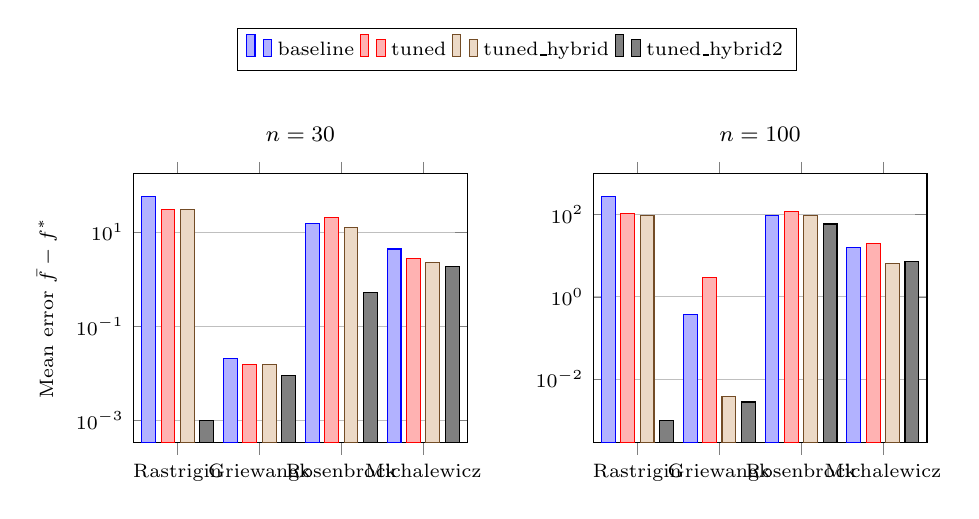
\begin{tikzpicture}
\begin{groupplot}[
  group style={group size=2 by 1, horizontal sep=1.6cm},
  ybar, width=0.48\textwidth, height=5cm,
  every axis plot/.append style={bar width=5pt},
  ymode=log, log origin=infty,
  symbolic x coords={Rastrigin,Griewangk,Rosenbrock,Michalewicz},
  xtick=data, enlarge x limits=0.18, ymajorgrids,
  tick label style={font=\scriptsize}, label style={font=\scriptsize},
  title style={font=\footnotesize, yshift=2pt},
  legend style={font=\scriptsize, at={(1.15,1.38)}, anchor=south, legend columns=4}]
\nextgroupplot[title={$n=30$}, ylabel={Mean error $\bar f-f^*$}]
\addplot coordinates {(Rastrigin,59.100) (Griewangk,0.0204) (Rosenbrock,15.617) (Michalewicz,4.414)};
\addplot coordinates {(Rastrigin,30.877) (Griewangk,0.0155) (Rosenbrock,20.548) (Michalewicz,2.735)};
\addplot coordinates {(Rastrigin,30.877) (Griewangk,0.0155) (Rosenbrock,12.910) (Michalewicz,2.319)};
\addplot coordinates {(Rastrigin,0.001) (Griewangk,0.0091) (Rosenbrock,0.535) (Michalewicz,1.856)};
\legend{baseline, tuned, tuned\_hybrid, tuned\_hybrid2}
\nextgroupplot[title={$n=100$}]
\addplot coordinates {(Rastrigin,281.644) (Griewangk,0.3657) (Rosenbrock,95.471) (Michalewicz,15.484)};
\addplot coordinates {(Rastrigin,106.767) (Griewangk,3.0028) (Rosenbrock,119.388) (Michalewicz,19.764)};
\addplot coordinates {(Rastrigin,93.924) (Griewangk,0.0038) (Rosenbrock,96.373) (Michalewicz,6.572)};
\addplot coordinates {(Rastrigin,0.001) (Griewangk,0.0028) (Rosenbrock,58.880) (Michalewicz,7.339)};
\end{groupplot}
\end{tikzpicture}
\caption{Mean error of the four variants on each function (log scale;
lower is better), for $n=30$ and $n=100$. The error is the mean result
minus the optimum. For Michalewicz the optimum is $\approx-29.63$ ($n=30$)
and $\approx-99.28$ ($n=100$). The tuned\_hybrid2 bar for Rastrigin is
drawn at $10^{-3}$ because its error is exactly 0, which a log axis cannot
show.}
\label{fig:var}
\end{figure*}

\textbf{Effect of tuning.} The tuned configuration reduces the Rastrigin
error by about 48\% in 30 dimensions and by 62\% in 100 dimensions, and
improves Michalewicz in 30 dimensions. These are the two functions where
small steps and particles that rely more on their own best than on the
group performed best in the parameter study. On Rosenbrock the tuned
variant is worse, which agrees with the study, where $(2.5,0.5)$ performed
poorly on that function. In 100 dimensions, tuning hurts Griewangk
($0.366\to3.00$) and Michalewicz. With $v_{\max}=0.05(b-a)$ the swarm moves
too slowly in 100 dimensions, particularly on the wide Griewangk domain,
and does not finish converging within the budget.

\textbf{Effect of hybridization.} The local search fixes exactly this
problem. In 100 dimensions it improves every one of the 30 runs on
Rastrigin, Griewangk and Michalewicz. It brings the Griewangk error down
from about 3 to 0.0038 and raises Michalewicz to $-92.71$, 93\% of the
best-known optimum, with a best run of $-95.44$. Coordinate search is
especially effective here because Michalewicz and Rastrigin are separable
and Griewangk is only weakly coupled. In 30 dimensions, by contrast, the
search finds nothing to improve on Rastrigin and Griewangk: the swarm has
already converged to a local minimum, and a coordinate step of $0.1$ cannot
cross the unit-spaced barriers of Rastrigin. On the non-separable
Rosenbrock, the search always exhausts its 20\,000-evaluation cap. It still
improves all runs and gives the best 30-dimensional result among the first
three variants (12.91). In 100 dimensions it brings the tuned variant back
to the baseline level (96.37), with a much smaller spread (std 9.21 versus
24.43). Fig.~\ref{fig:box} and Fig.~\ref{fig:conv_var} show the run
distributions and the convergence curves; the final jump in the hybrid
curves corresponds to the local search.

\textbf{Effect of the enhanced hybrid (tuned\_hybrid2).} Adding a larger
swarm, stagnation restarts, crossover and a stronger local search changes
the picture. Rastrigin is now solved exactly in both 30 and 100 dimensions
(mean $0.0$, std $0.0$), because the restart repeatedly injects diversity
and the coordinate search pushes each variable to the nearest whole number,
which is exactly where Rastrigin's lowest points are. On Rosenbrock the
crossover recombines good coordinates and follows the valley far better:
the mean drops from 15.62 to 0.53 in 30 dimensions and from 95.47 to 58.88
in 100 dimensions. Michalewicz improves to $-27.77$ in 30 dimensions and
reaches 93\% of the best-known value in 100 dimensions ($-91.94$, best run
$-95.35$). Griewangk also improves ($0.0091$ in 30 dimensions, $0.0028$ in
100). Every difference with respect to the baseline is reliable
($p<10^{-5}$ in most cases, $p<0.05$ everywhere). The one trade-off is in
100-dimensional Michalewicz, where the mean is slightly behind
tuned\_hybrid ($-91.94$ versus $-92.71$): there the restart occasionally
discards good plateaus before the swarm can exploit them.

\textbf{Cost.} The enhanced hybrid is markedly more expensive than the
other variants, because of its larger swarm and its much longer local
search. On 100-dimensional problems it uses roughly twice as many
evaluations as the baseline (for example about $626\,000$ on Rosenbrock
against $300\,050$), and its running time per run rises from a few seconds
to several minutes on the hardest instances. The gain in accuracy therefore
comes at a clear cost in computation.

\begin{figure*}[!t]
\centering
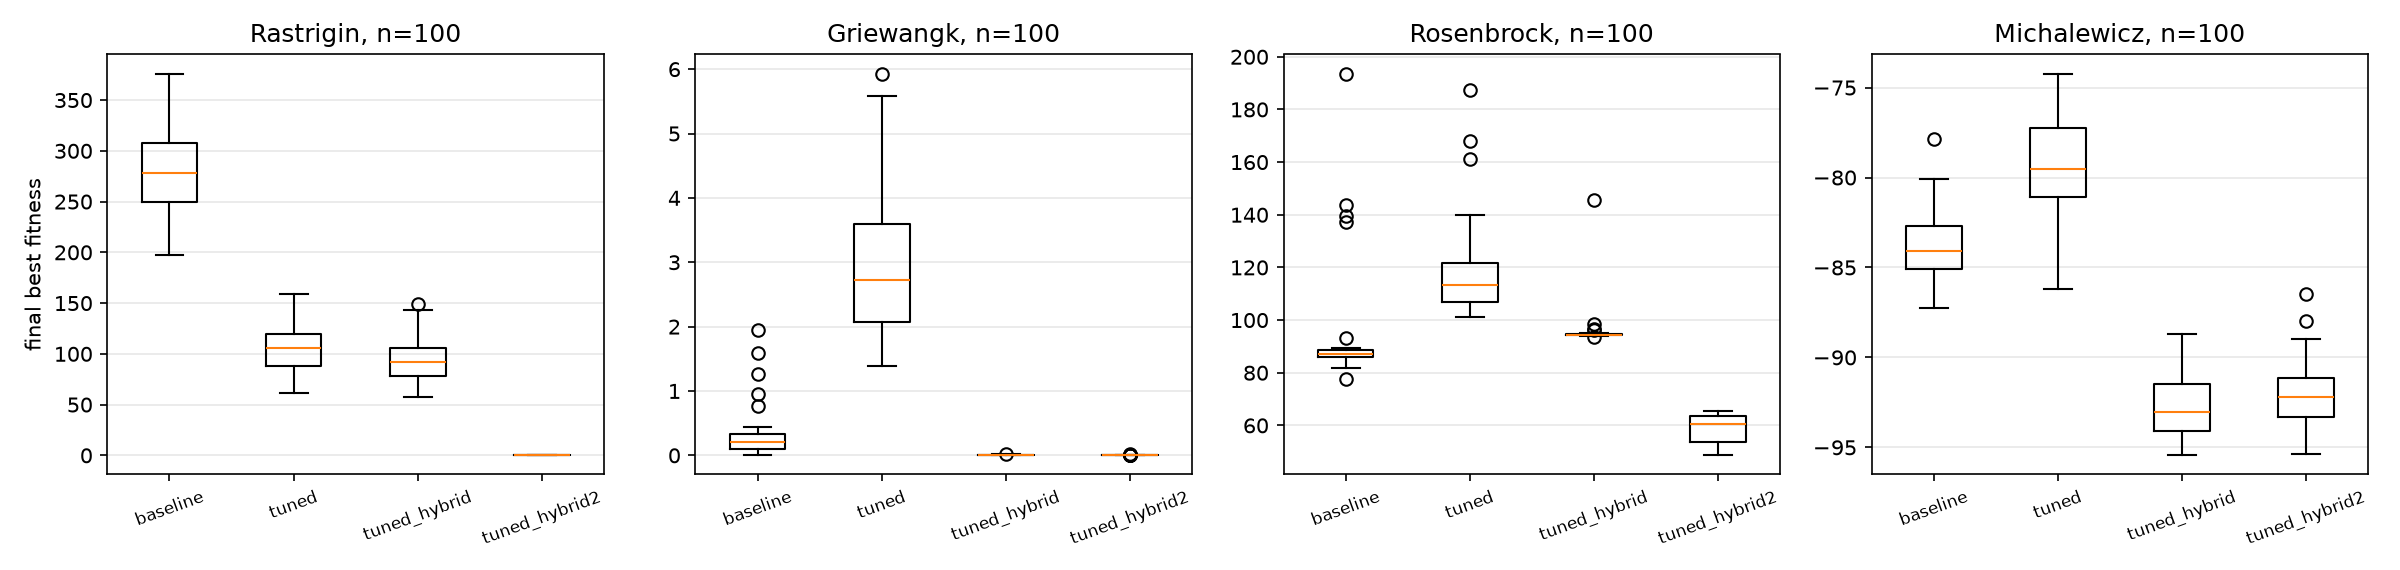
\includegraphics[width=\textwidth]{grafice_pso/boxplot_variants_n100.png}
\caption{Distribution of final values over 30 runs for the four variants,
$n=100$.}
\label{fig:box}
\end{figure*}

\begin{figure*}[!t]
\centering
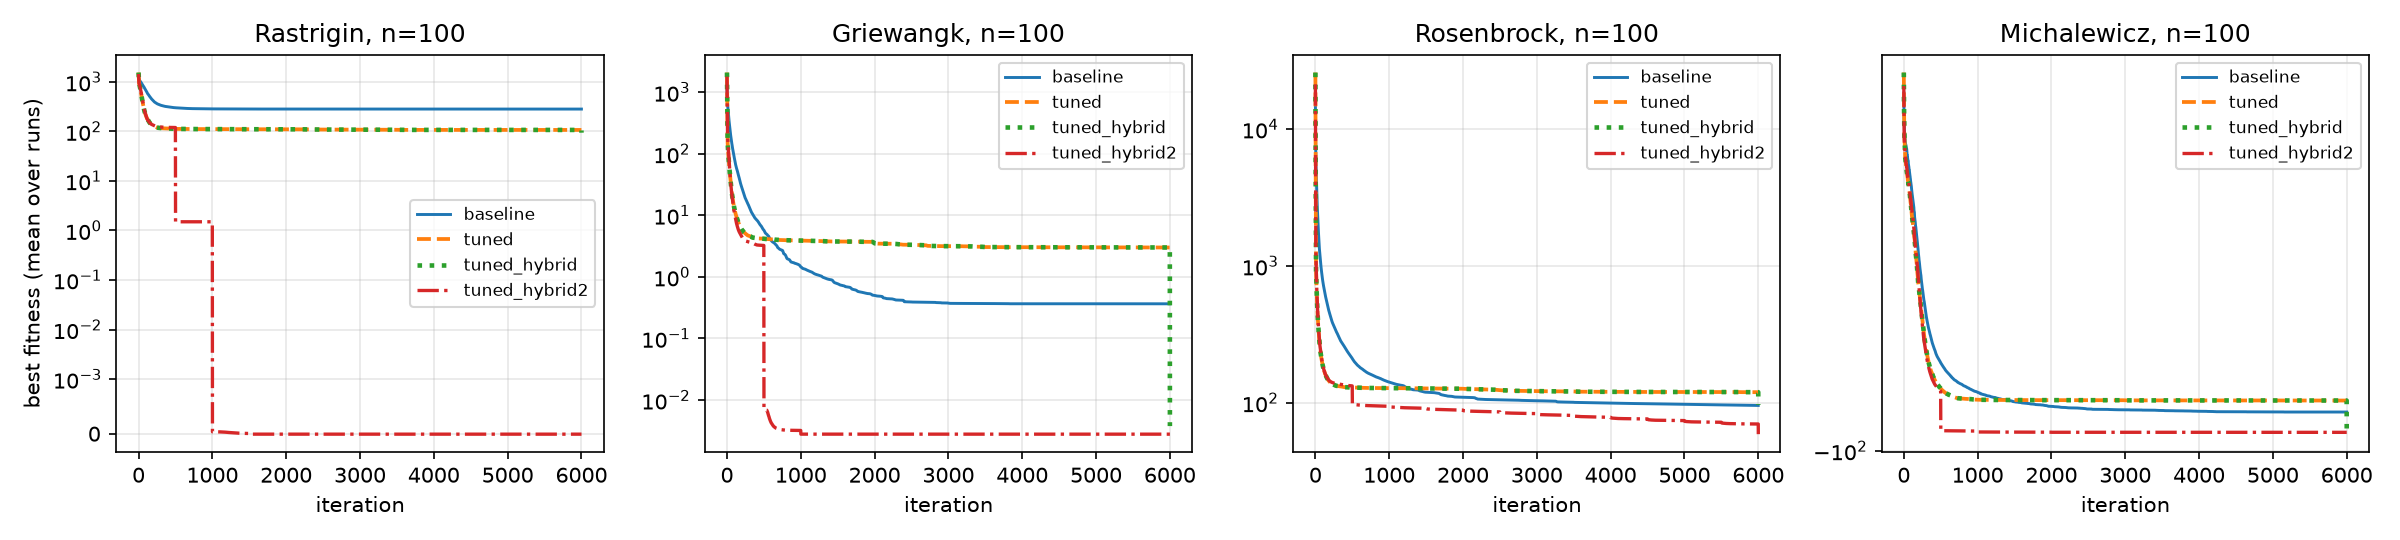
\includegraphics[width=\textwidth]{grafice_pso/convergence_variants_n100.png}
\caption{Mean convergence of the four variants, $n=100$. The last point of
the hybrid curves is the result after local search.}
\label{fig:conv_var}
\end{figure*}

\subsection{Comparison with HC and GA (H1)}
Table~\ref{tab:cmp} compares the mean results of PSO with those of the
binary Hill Climbing (HC) and of the binary GA hybridized with HC from H1.
Fig.~\ref{fig:cmp30} and Fig.~\ref{fig:cmp100} show the same data
graphically. HC was not run in 100 dimensions in H1 because of its cost.

\begin{table}[t]
\centering
\caption{Mean best value (30 runs): HC and GA+HC (H1) versus baseline PSO
and the enhanced hybrid PSO (tuned\_hybrid2). Best per row in bold.}
\label{tab:cmp}
\setlength{\tabcolsep}{3pt}
\begin{tabular}{llrrrr}
\toprule
Function & $n$ & HC & GA+HC & PSO & PSO hybrid2\\
\midrule
Rastrigin   & 2   & \textbf{0.000} & \textbf{0.000} & \textbf{0.000} & \textbf{0.000}\\
Griewangk   & 2   & 0.002 & 0.004 & 0.001 & \textbf{0.000}\\
Rosenbrock  & 2   & 0.000 & \textbf{0.000} & \textbf{0.000} & \textbf{0.000}\\
Michalewicz & 2   & $\mathbf{-1.801}$ & $\mathbf{-1.801}$ & $\mathbf{-1.801}$ & $\mathbf{-1.801}$\\
\midrule
Rastrigin   & 30  & 44.366 & 19.899 & 59.100 & \textbf{0.000}\\
Griewangk   & 30  & \textbf{0.000} & \textbf{0.000} & 0.020 & 0.009\\
Rosenbrock  & 30  & 35.477 & \textbf{0.000} & 15.617 & 0.535\\
Michalewicz & 30  & $-25.424$ & $-26.327$ & $-25.216$ & $\mathbf{-27.774}$\\
\midrule
Rastrigin   & 100 & --    & 185.991 & 281.644 & \textbf{0.000}\\
Griewangk   & 100 & --    & 0.072 & 0.366 & \textbf{0.003}\\
Rosenbrock  & 100 & --    & \textbf{0.000} & 95.471 & 58.880\\
Michalewicz & 100 & --    & $-84.971$ & $-83.796$ & $\mathbf{-91.941}$\\
\bottomrule
\end{tabular}
\end{table}

\begin{figure*}[!t]
\centering
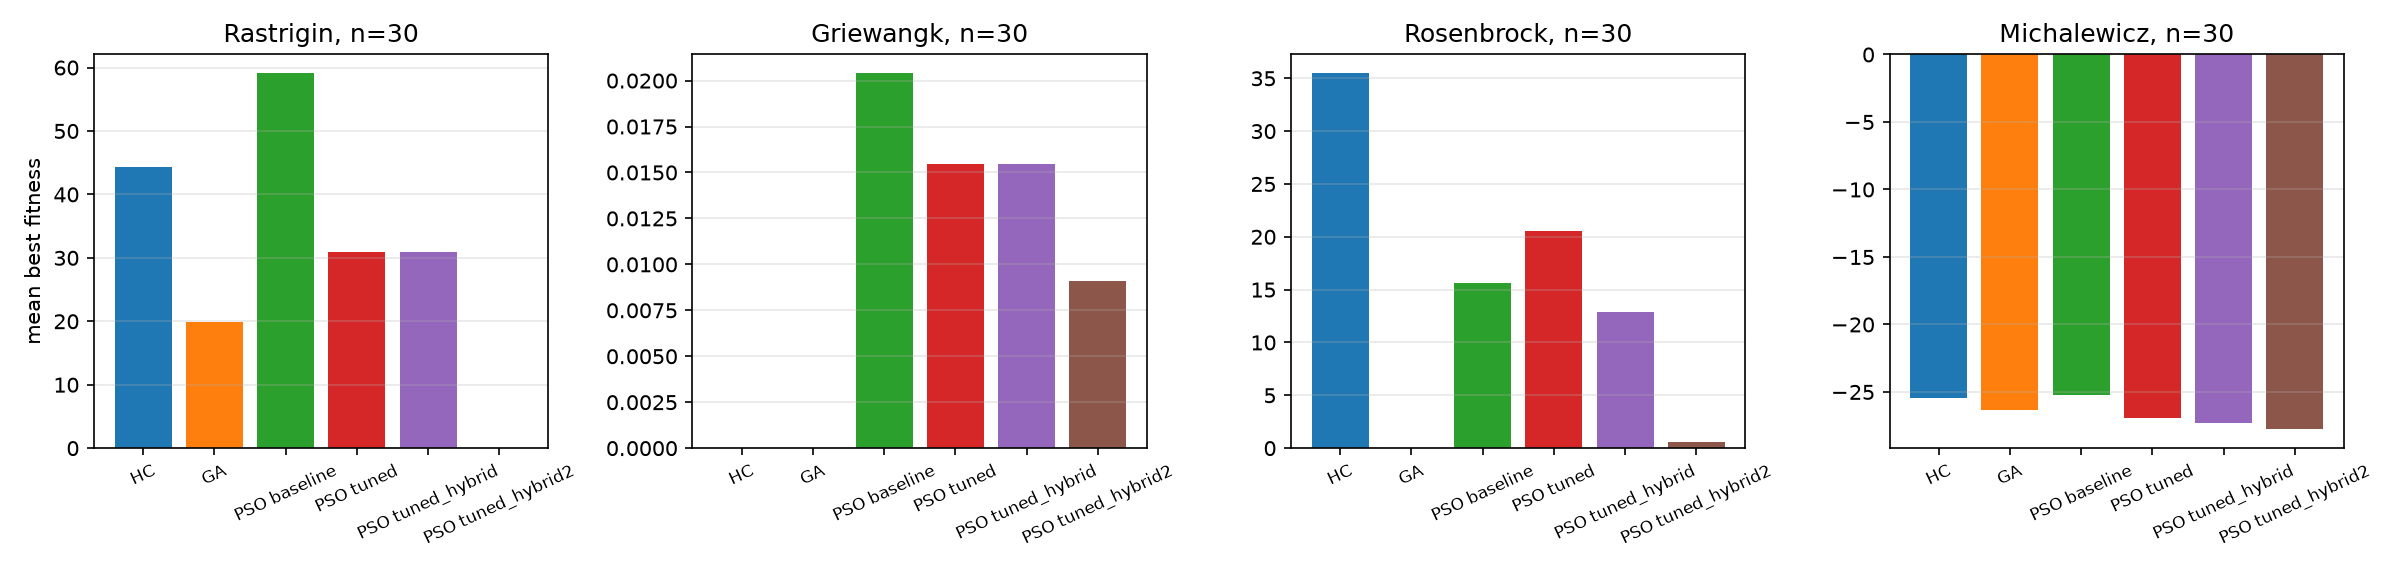
\includegraphics[width=\textwidth]{grafice_pso/comparison_h1_n30.png}
\caption{Mean best value of HC, GA+HC (H1), PSO and the enhanced hybrid PSO, $n=30$.}
\label{fig:cmp30}
\end{figure*}

\begin{figure*}[!t]
\centering
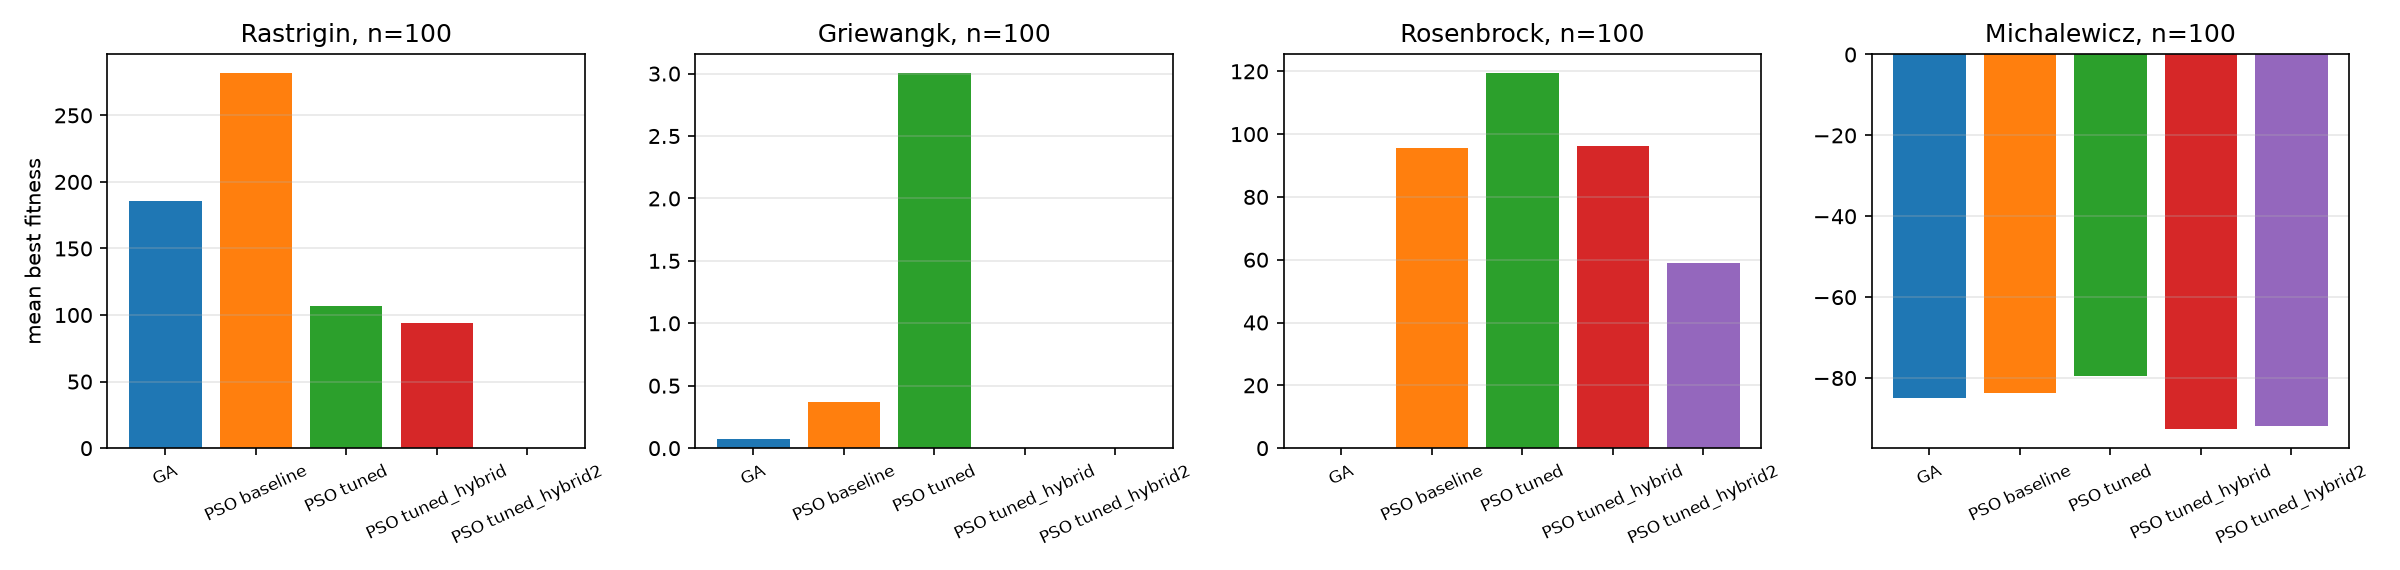
\includegraphics[width=\textwidth]{grafice_pso/comparison_h1_n100.png}
\caption{Mean best value of GA+HC (H1), PSO and the enhanced hybrid PSO, $n=100$.}
\label{fig:cmp100}
\end{figure*}

\textbf{Two dimensions.} All methods find the global optimum of
Rastrigin, Rosenbrock and Michalewicz. On Griewangk, the hybrid PSO is the
only method whose mean is 0.000; HC and GA+HC occasionally stop in a
neighboring local minimum.

\textbf{Thirty dimensions.} The enhanced hybrid PSO (tuned\_hybrid2) is now
the strongest method on three of the four functions. It solves Rastrigin
exactly (0.000 versus 19.90 for GA+HC), wins on Michalewicz ($-27.77$
versus $-26.33$), and brings Rosenbrock down to 0.53, far below plain HC
(35.48) and baseline PSO (15.62), though GA+HC still reaches 0.000. On
Griewangk all methods are essentially tied near zero. Plain HC is better
than baseline PSO on Rastrigin (44.37 versus 59.10) because its restarts
sample many basins, but worse on Rosenbrock.

\textbf{One hundred dimensions.} In 100 dimensions the enhanced hybrid PSO
obtains the best mean on three of the four functions: Rastrigin (0.000
versus 185.99 for GA+HC), Griewangk (0.003 versus 0.072) and Michalewicz
($-91.94$ versus $-84.97$, 93\% versus 86\% of the best-known optimum). On
Rosenbrock it reduces the baseline error from 95.47 to 58.88, but GA+HC
remains clearly superior there (0.000), thanks to its exhaustive bit-flip
local search.

\textbf{Why GA+HC excels on Rosenbrock.} The binary HC used in H1 examines,
at each step, all $n\cdot L$ bit-flip neighbors and moves to the best one.
Flipping a high-order bit produces a large jump on one variable, while
flipping a low-order bit produces a move at the level of the fifth
decimal. This exhaustive, multi-scale neighborhood is well suited to
following the narrow Rosenbrock valley, at a high cost in evaluations. In
contrast, the coordinate search used in the hybrid PSO starts from a
single step size and is limited to 20\,000 evaluations, a limit that was
always reached on Rosenbrock.

\textbf{Why PSO scales better on multimodal functions.} The swarm
explores with real-valued, continuous moves and shares information among
all particles. A binary GA, whether using standard or Gray
coding~\cite{caruana1988}, must search a space of $n\cdot L$ bits, more
than 2\,000 bits for $n=100$, where crossover and mutation become less
effective as the string length grows.

\textbf{Cost.} A 30-dimensional baseline PSO run takes 0.4--0.7\,s and a
100-dimensional run about 4\,s, since PSO works directly on real vectors
and needs no binary decoding. The enhanced hybrid is slower because of its
longer local search, but still far cheaper than the binary methods of H1,
which must decode every candidate and evaluate $n\cdot L$ bit-flip
neighbors at each HC step.

%=====================================================================
\FloatBarrier
\section{Discussion}\label{sec:discussion}
%=====================================================================
\textbf{Exploration versus exploitation.} Every parameter we studied
controls the same balance: searching widely versus digging deep in one
spot. Inertia sets how much a particle keeps moving, the coefficients set
how strongly it is pulled and towards what, $v_{\max}$ sets how big a step
can be, and the topology sets how fast good news spreads. The best settings
sit right at the edge where the swarm still settles down but keeps enough
energy to explore.

\textbf{No single setting fits all.} Rastrigin likes settings that keep the
swarm spread out (small $v_{\max}$, a larger $c_1$ than $c_2$, ring
topology, decreasing inertia), while Griewangk and Rosenbrock like fast
teamwork (global topology, equal coefficients). As the No Free Lunch
theorem~\cite{wolpert1997} says, no setting can win everywhere: the tuned
configuration helps the functions it was made for and hurts Rosenbrock.

\textbf{Dimension and budget.} The best settings at $n=30$ do not carry
over to $n=100$. A small step size that helps at 30 dimensions is too slow
at 100. Giving more iterations helps smooth functions like Rosenbrock, but
does not help Rastrigin, where the swarm is simply stuck.

\textbf{Hybridization.} Pairing a wide-searching swarm with a local
search makes up for the swarm's slow finish. Adding a larger swarm,
restarts and crossover, as in the enhanced hybrid, gives the best mean in
almost every high-dimensional case, at the price of more evaluations. This
is the same lesson as in H1, where adding HC to the GA improved precision.

\textbf{PSO versus GA+HC.} Neither method wins everywhere. GA+HC stays
ahead on Rosenbrock, thanks to its thorough bit-flip local search. The
enhanced hybrid PSO matches or beats GA+HC on the multimodal functions in
both 30 and 100 dimensions. A good next step is to give the PSO hybrid a
stronger local search like the one in H1 to fix Rosenbrock, and to try PSO
versions built for multimodal functions, such as the comprehensive learning
PSO~\cite{liang2006}.

\textbf{Limitations.} The parameter study uses only 10 runs, so small
differences (less than one standard deviation) should not be trusted too
much. We changed one parameter at a time, so we did not measure how
parameters interact. The enhanced hybrid also uses noticeably more
evaluations than the others.

%=====================================================================
\FloatBarrier
\section{Conclusion}\label{sec:conclusion}
%=====================================================================
A PSO that works directly on real numbers, with a limit on how fast
particles can move, adjustable inertia and a global or ring topology was
built and tested on four functions in 2, 30 and 100 dimensions. PSO solves
every 2D case exactly. The parameter study shows that the inertia weight and
the balance between the two coefficients matter most, and their effect
matches the known stability condition. Dropping the social term is the
worst choice, a small step size is the single most useful change on the
multimodal functions, and the best topology and inertia schedule depend on
the function. Using these findings, we built a tuned PSO, a hybrid PSO with
a local search at the end, and an enhanced hybrid that also adds a larger
swarm, restarts, crossover and a stronger local search. The enhanced hybrid
reaches the optimum of Rastrigin in 30 and 100 dimensions, cuts the
30-dimensional Rosenbrock error from 15.6 to 0.53 and the 100-dimensional
one from 95.5 to 58.9, and gets to 93\% of the best-known value on
100-dimensional Michalewicz. It improves the baseline clearly on every
function, at the price of more evaluations.

Compared with the methods of H1, the enhanced hybrid PSO is as good or
better than GA+HC on functions with many local minima, in both 30 and 100
dimensions. GA+HC stays clearly ahead only on Rosenbrock, thanks to its
thorough bit-flip local search.

\FloatBarrier

\begin{thebibliography}{00}
\bibitem{kennedy1995} J. Kennedy and R. Eberhart, ``Particle swarm
optimization,'' in \textit{Proc. IEEE Int. Conf. Neural Networks (ICNN'95)},
vol.~4, 1995, pp.~1942--1948.
\bibitem{eberhart1995} R. Eberhart and J. Kennedy, ``A new optimizer using
particle swarm theory,'' in \textit{Proc. 6th Int. Symp. Micro Machine and
Human Science (MHS'95)}, 1995, pp.~39--43.
\bibitem{holland1975} J. H. Holland, \textit{Adaptation in Natural and
Artificial Systems}. Ann Arbor, MI, USA: Univ. of Michigan Press, 1975.
\bibitem{goldberg1989} D. E. Goldberg, \textit{Genetic Algorithms in Search,
Optimization, and Machine Learning}. Reading, MA, USA: Addison-Wesley, 1989.
\bibitem{kennedy2001} J. Kennedy, R. C. Eberhart, and Y. Shi,
\textit{Swarm Intelligence}. San Francisco, CA, USA: Morgan Kaufmann, 2001.
\bibitem{poli2007} R. Poli, J. Kennedy, and T. Blackwell, ``Particle swarm
optimization: An overview,'' \textit{Swarm Intelligence}, vol.~1, no.~1,
pp.~33--57, 2007.
\bibitem{engelbrecht2007} A. P. Engelbrecht, \textit{Computational
Intelligence: An Introduction}, 2nd~ed. Chichester, U.K.: Wiley, 2007.
\bibitem{bonyadi2017} M. R. Bonyadi and Z. Michalewicz, ``Particle swarm
optimization for single objective continuous space problems: A review,''
\textit{Evolutionary Computation}, vol.~25, no.~1, pp.~1--54, 2017.
\bibitem{angeline1998} P. J. Angeline, ``Evolutionary optimization versus
particle swarm optimization: Philosophy and performance differences,'' in
\textit{Evolutionary Programming VII}, LNCS vol.~1447. Berlin, Germany:
Springer, 1998, pp.~601--610.
\bibitem{michalewicz1996} Z. Michalewicz, \textit{Genetic Algorithms + Data
Structures = Evolution Programs}, 3rd~ed. Berlin, Germany: Springer, 1996.
\bibitem{talbi2002} E.-G. Talbi, ``A taxonomy of hybrid metaheuristics,''
\textit{Journal of Heuristics}, vol.~8, no.~5, pp.~541--564, 2002.
\bibitem{geatbx} H. Pohlheim, ``GEATbx: Example functions (single and
multi-objective functions),'' [Online]. Available:
http://www.geatbx.com/docu/fcnindex-01.html
\bibitem{jamil2013} M. Jamil and X.-S. Yang, ``A literature survey of
benchmark functions for global optimisation problems,'' \textit{Int. J.
Mathematical Modelling and Numerical Optimisation}, vol.~4, no.~2,
pp.~150--194, 2013.
\bibitem{rastrigin1974} L. A. Rastrigin, \textit{Systems of Extremal
Control}. Moscow, USSR: Nauka, 1974 (in Russian).
\bibitem{muhlenbein1991} H. M\"{u}hlenbein, M. Schomisch, and J. Born, ``The
parallel genetic algorithm as function optimizer,'' \textit{Parallel
Computing}, vol.~17, no.~6--7, pp.~619--632, 1991.
\bibitem{griewank1981} A. O. Griewank, ``Generalized descent for global
optimization,'' \textit{Journal of Optimization Theory and Applications},
vol.~34, no.~1, pp.~11--39, 1981.
\bibitem{rosenbrock1960} H. H. Rosenbrock, ``An automatic method for finding
the greatest or least value of a function,'' \textit{The Computer Journal},
vol.~3, no.~3, pp.~175--184, 1960.
\bibitem{shi1998} Y. Shi and R. Eberhart, ``A modified particle swarm
optimizer,'' in \textit{Proc. IEEE Int. Conf. Evolutionary Computation},
1998, pp.~69--73.
\bibitem{shi1999} Y. Shi and R. C. Eberhart, ``Empirical study of particle
swarm optimization,'' in \textit{Proc. Congress on Evolutionary Computation
(CEC'99)}, vol.~3, 1999, pp.~1945--1950.
\bibitem{kennedy2002} J. Kennedy and R. Mendes, ``Population structure and
particle swarm performance,'' in \textit{Proc. Congress on Evolutionary
Computation (CEC'02)}, 2002, pp.~1671--1676.
\bibitem{mendes2004} R. Mendes, J. Kennedy, and J. Neves, ``The fully
informed particle swarm: Simpler, maybe better,'' \textit{IEEE Trans. Evol.
Comput.}, vol.~8, no.~3, pp.~204--210, 2004.
\bibitem{clerc2002} M. Clerc and J. Kennedy, ``The particle swarm --
explosion, stability, and convergence in a multidimensional complex
space,'' \textit{IEEE Trans. Evol. Comput.}, vol.~6, no.~1, pp.~58--73,
2002.
\bibitem{eberhart2000} R. C. Eberhart and Y. Shi, ``Comparing inertia weights
and constriction factors in particle swarm optimization,'' in \textit{Proc.
Congress on Evolutionary Computation (CEC'00)}, vol.~1, 2000, pp.~84--88.
\bibitem{shi1998param} Y. Shi and R. C. Eberhart, ``Parameter selection in
particle swarm optimization,'' in \textit{Evolutionary Programming VII},
LNCS vol.~1447. Berlin, Germany: Springer, 1998, pp.~591--600.
\bibitem{poli2009} R. Poli, ``Mean and variance of the sampling
distribution of particle swarm optimizers during stagnation,''
\textit{IEEE Trans. Evol. Comput.}, vol.~13, no.~4, pp.~712--721, 2009.
\bibitem{trelea2003} I. C. Trelea, ``The particle swarm optimization
algorithm: Convergence analysis and parameter selection,''
\textit{Information Processing Letters}, vol.~85, no.~6, pp.~317--325, 2003.
\bibitem{vandenbergh2006} F. van den Bergh and A. P. Engelbrecht, ``A study
of particle swarm optimization particle trajectories,'' \textit{Information
Sciences}, vol.~176, no.~8, pp.~937--971, 2006.
\bibitem{hooke1961} R. Hooke and T. A. Jeeves, ```Direct search' solution of
numerical and statistical problems,'' \textit{Journal of the ACM}, vol.~8,
no.~2, pp.~212--229, 1961.
\bibitem{harris2020} C. R. Harris \textit{et al.}, ``Array programming with
NumPy,'' \textit{Nature}, vol.~585, no.~7825, pp.~357--362, 2020.
\bibitem{hunter2007} J. D. Hunter, ``Matplotlib: A 2D graphics
environment,'' \textit{Computing in Science \& Engineering}, vol.~9, no.~3,
pp.~90--95, 2007.
\bibitem{mann1947} H. B. Mann and D. R. Whitney, ``On a test of whether one
of two random variables is stochastically larger than the other,''
\textit{Annals of Mathematical Statistics}, vol.~18, no.~1, pp.~50--60,
1947.
\bibitem{derrac2011} J. Derrac, S. Garc\'{i}a, D. Molina, and F. Herrera,
``A practical tutorial on the use of nonparametric statistical tests as a
methodology for comparing evolutionary and swarm intelligence
algorithms,'' \textit{Swarm and Evolutionary Computation}, vol.~1, no.~1,
pp.~3--18, 2011.
\bibitem{ratnaweera2004} A. Ratnaweera, S. K. Halgamuge, and H. C. Watson,
``Self-organizing hierarchical particle swarm optimizer with time-varying
acceleration coefficients,'' \textit{IEEE Trans. Evol. Comput.}, vol.~8,
no.~3, pp.~240--255, 2004.
\bibitem{bratton2007} D. Bratton and J. Kennedy, ``Defining a standard for
particle swarm optimization,'' in \textit{Proc. IEEE Swarm Intelligence
Symposium}, 2007, pp.~120--127.
\bibitem{caruana1988} R. A. Caruana and J. D. Schaffer, ``Representation and
hidden bias: Gray vs. binary coding for genetic algorithms,'' in
\textit{Proc. 5th Int. Conf. Machine Learning}, 1988, pp.~153--161.
\bibitem{wolpert1997} D. H. Wolpert and W. G. Macready, ``No free lunch
theorems for optimization,'' \textit{IEEE Trans. Evol. Comput.}, vol.~1,
no.~1, pp.~67--82, 1997.
\bibitem{liang2006} J. J. Liang, A. K. Qin, P. N. Suganthan, and S. Baskar,
``Comprehensive learning particle swarm optimizer for global optimization
of multimodal functions,'' \textit{IEEE Trans. Evol. Comput.}, vol.~10,
no.~3, pp.~281--295, 2006.
\end{thebibliography}

\end{document}
